% Generated by experiments/paper/fig_clotho_vs_lookup.py; do not edit.
\begin{figure*}[t]
\centering
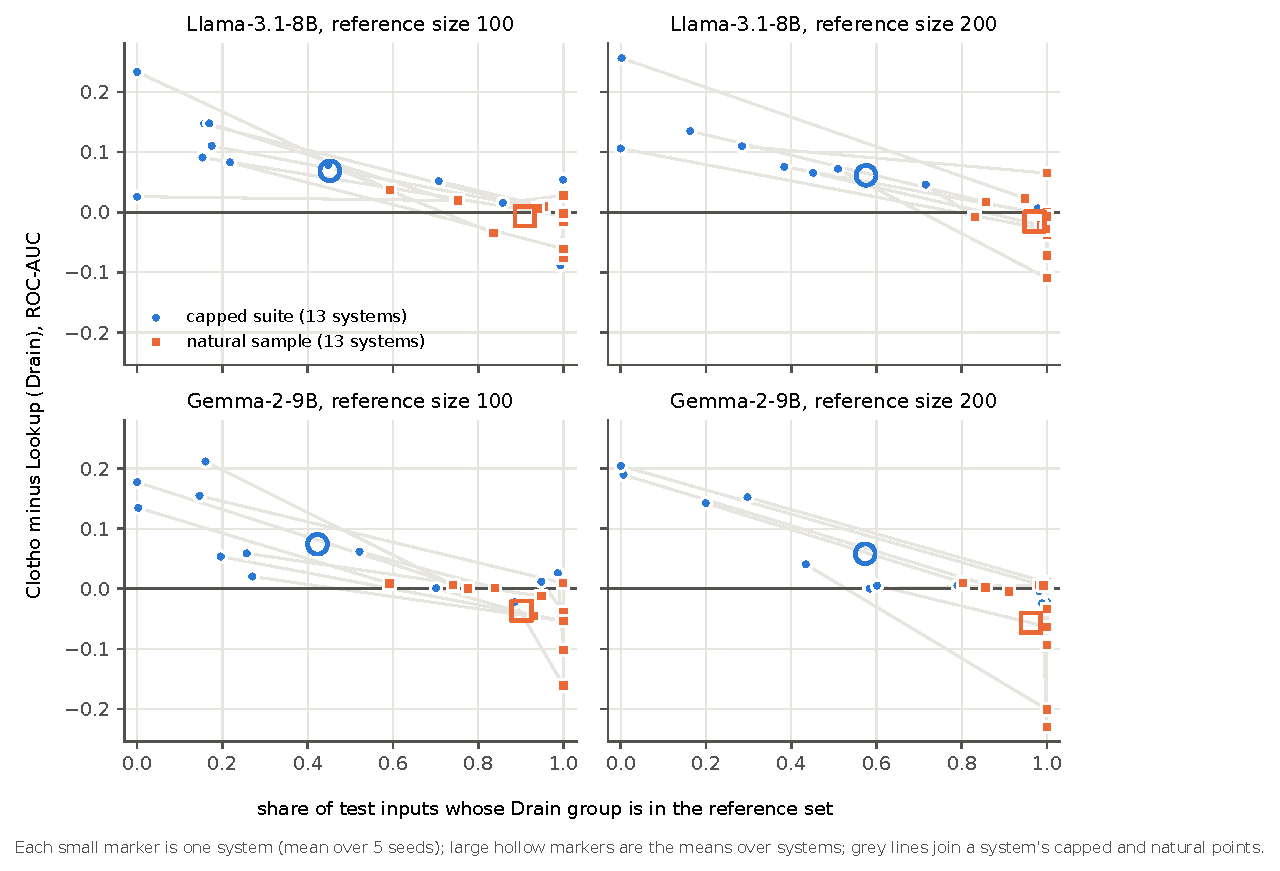
\includegraphics[width=\textwidth]{figures/clotho_vs_lookup.pdf}
\caption{Clotho minus Lookup (Drain), per system, against the share of test inputs whose Drain group already occurs among the non-initial reference inputs; template-capped suites (circles) vs natural samples (squares), both models, standard split, reference sizes 100 and 200. Small markers: one system, mean over 5 seeds; large hollow markers: mean over systems; grey lines join a system's two points. Drain with the Loghub-2.0 benchmark settings, run on each suite's 500 messages. Systems: Llama 13 capped / 13 natural, Gemma 12 / 12. fair\_leakfree setting: balanced reference sampling, hidden layer 16 (Llama) / 21 (Gemma) for Clotho, MDSA and GMMb, pass label from samples 5--9 (PASS if $\geq$3 of 5 strict template matches), post-generation scores from samples 0--4; rules\_template prompt, strict match. ROC-AUC, mean $\pm$ std over 5 seeds of the per-seed macro mean over systems. Reference size includes the 10 initial tests. $^*$ needs the generated outputs.}
\label{fig:clotho-vs-lookup}
\end{figure*}
